\subsection{Electrolysis}
\begin{frame}
\frametitle{Electrolysis}
\begin{columns}
    \column[t]{5cm}
	\begin{figure}[htbp!]
		\begin{center}
			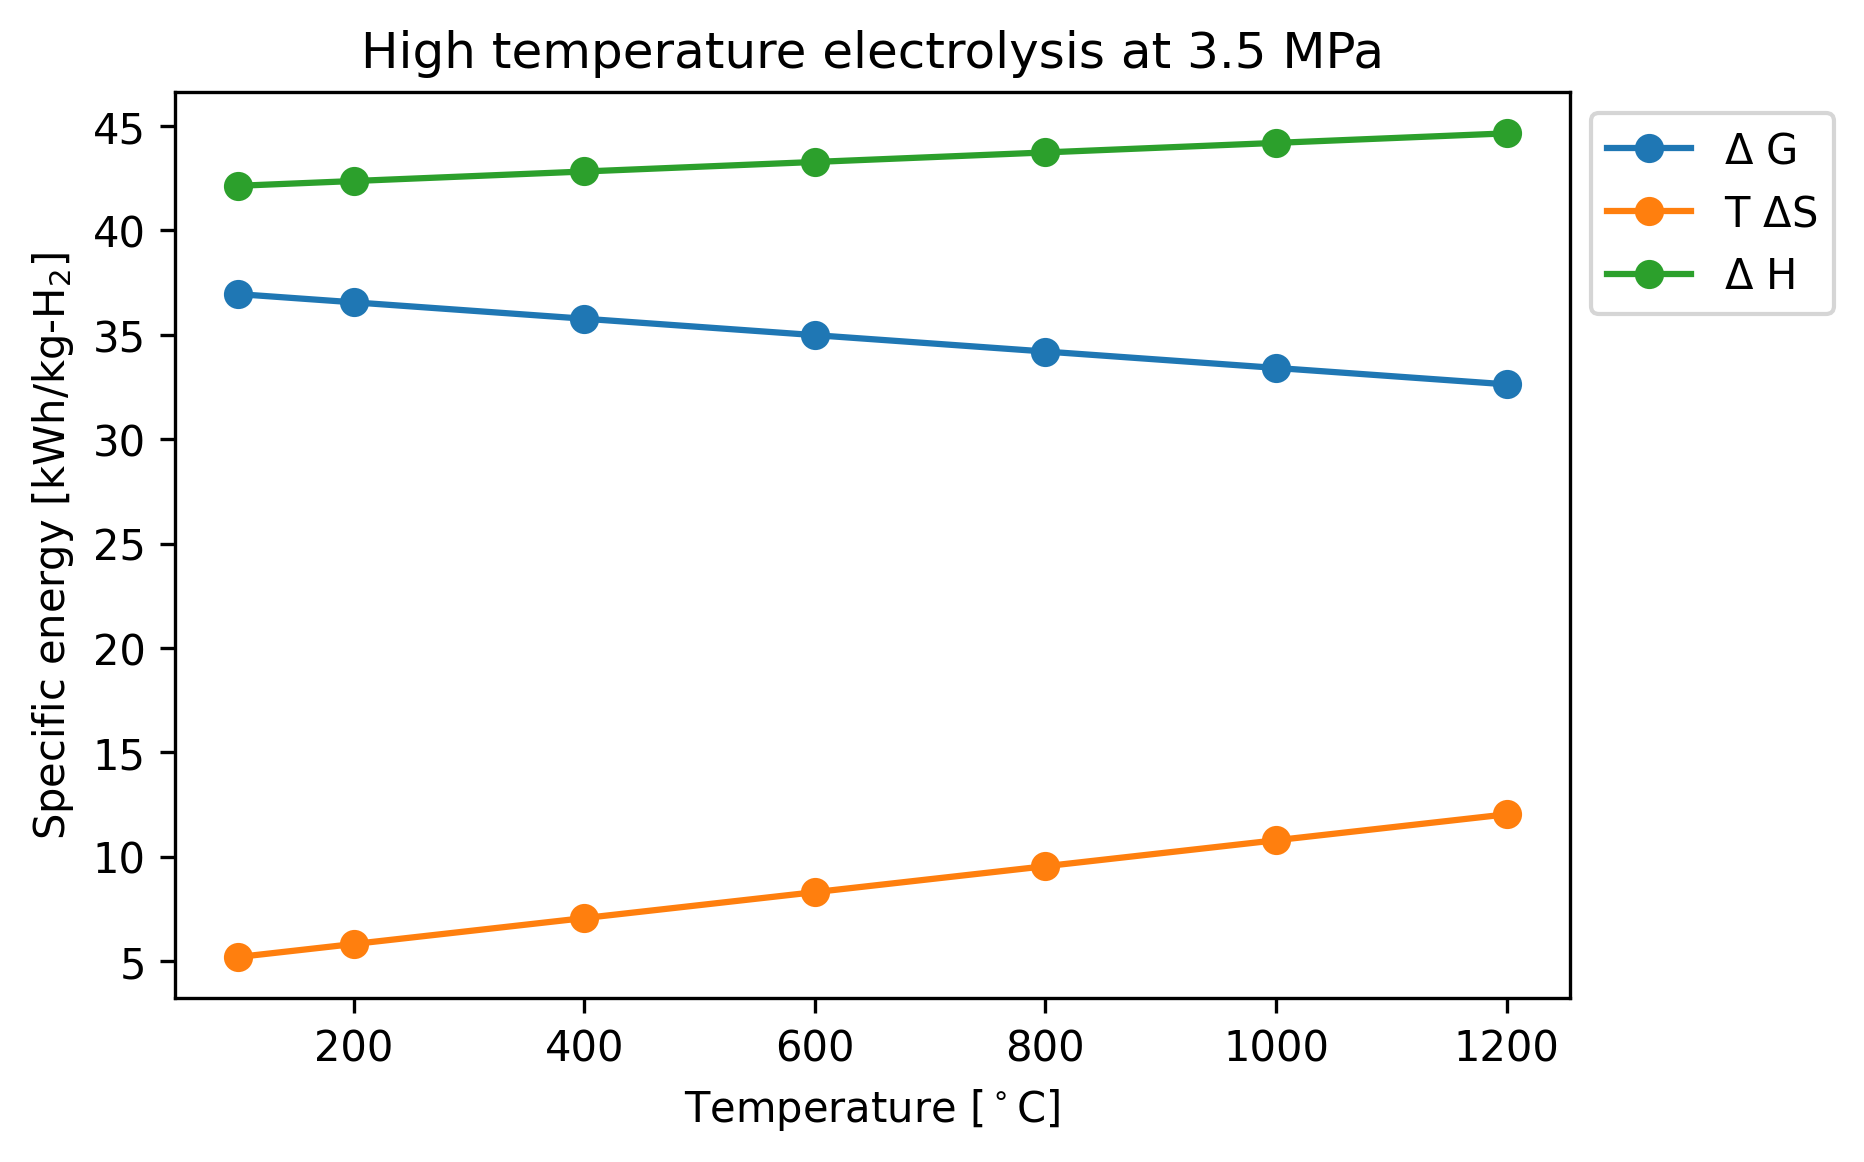
\includegraphics[height=3.6cm]{images/hte-energy-P.png}
		\end{center}
		\caption{Energy required by HTE at 3.5 MPa.}
	\end{figure}

	\column[t]{5cm}
	$\Delta H = \Delta G + T \Delta S$
	\begin{itemize}
		\item $\Delta$G: specific electrical energy $kWh \cdot kg_{H_2}^{-1}$
		\item T$\Delta$S: specific thermal energy $kWh \cdot kg_{H_2}^{-1}$.
	\end{itemize}
    \vspace{0.7cm}

	\begin{itemize}
    	\item In low temperature electrolysis (LTE), electricity provides the thermal energy.
    	\item In high temperature electrolysis (HTE), a heat source provides the thermal energy.
    	\item HTE has the advantage of decreasing the electricity requirement.
    \end{itemize}
\end{columns}
\end{frame}

\subsection{Sulfur-Iodine}
\begin{frame}
\frametitle{Sulfur-Iodine}
\begin{columns}
    \column[t]{5cm}
  	\begin{figure}[htbp!]
		\begin{center}
			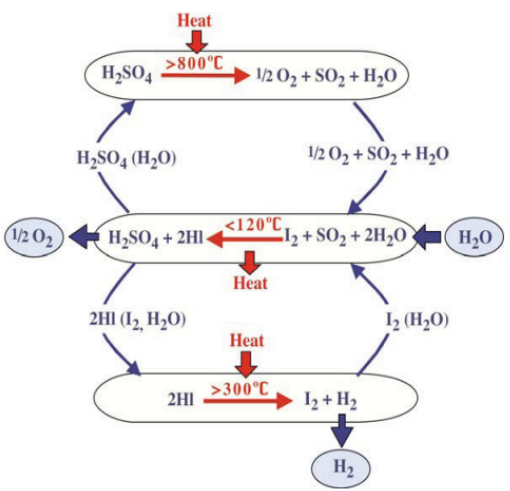
\includegraphics[width=5cm]{images/sulfur1.png}
		\end{center}
		\caption{Diagram of the Sulfur-Iodine Thermochemical process.}
 	\end{figure}

 	\column[t]{5cm}
   	\begin{figure}[htbp!]
		\begin{center}
			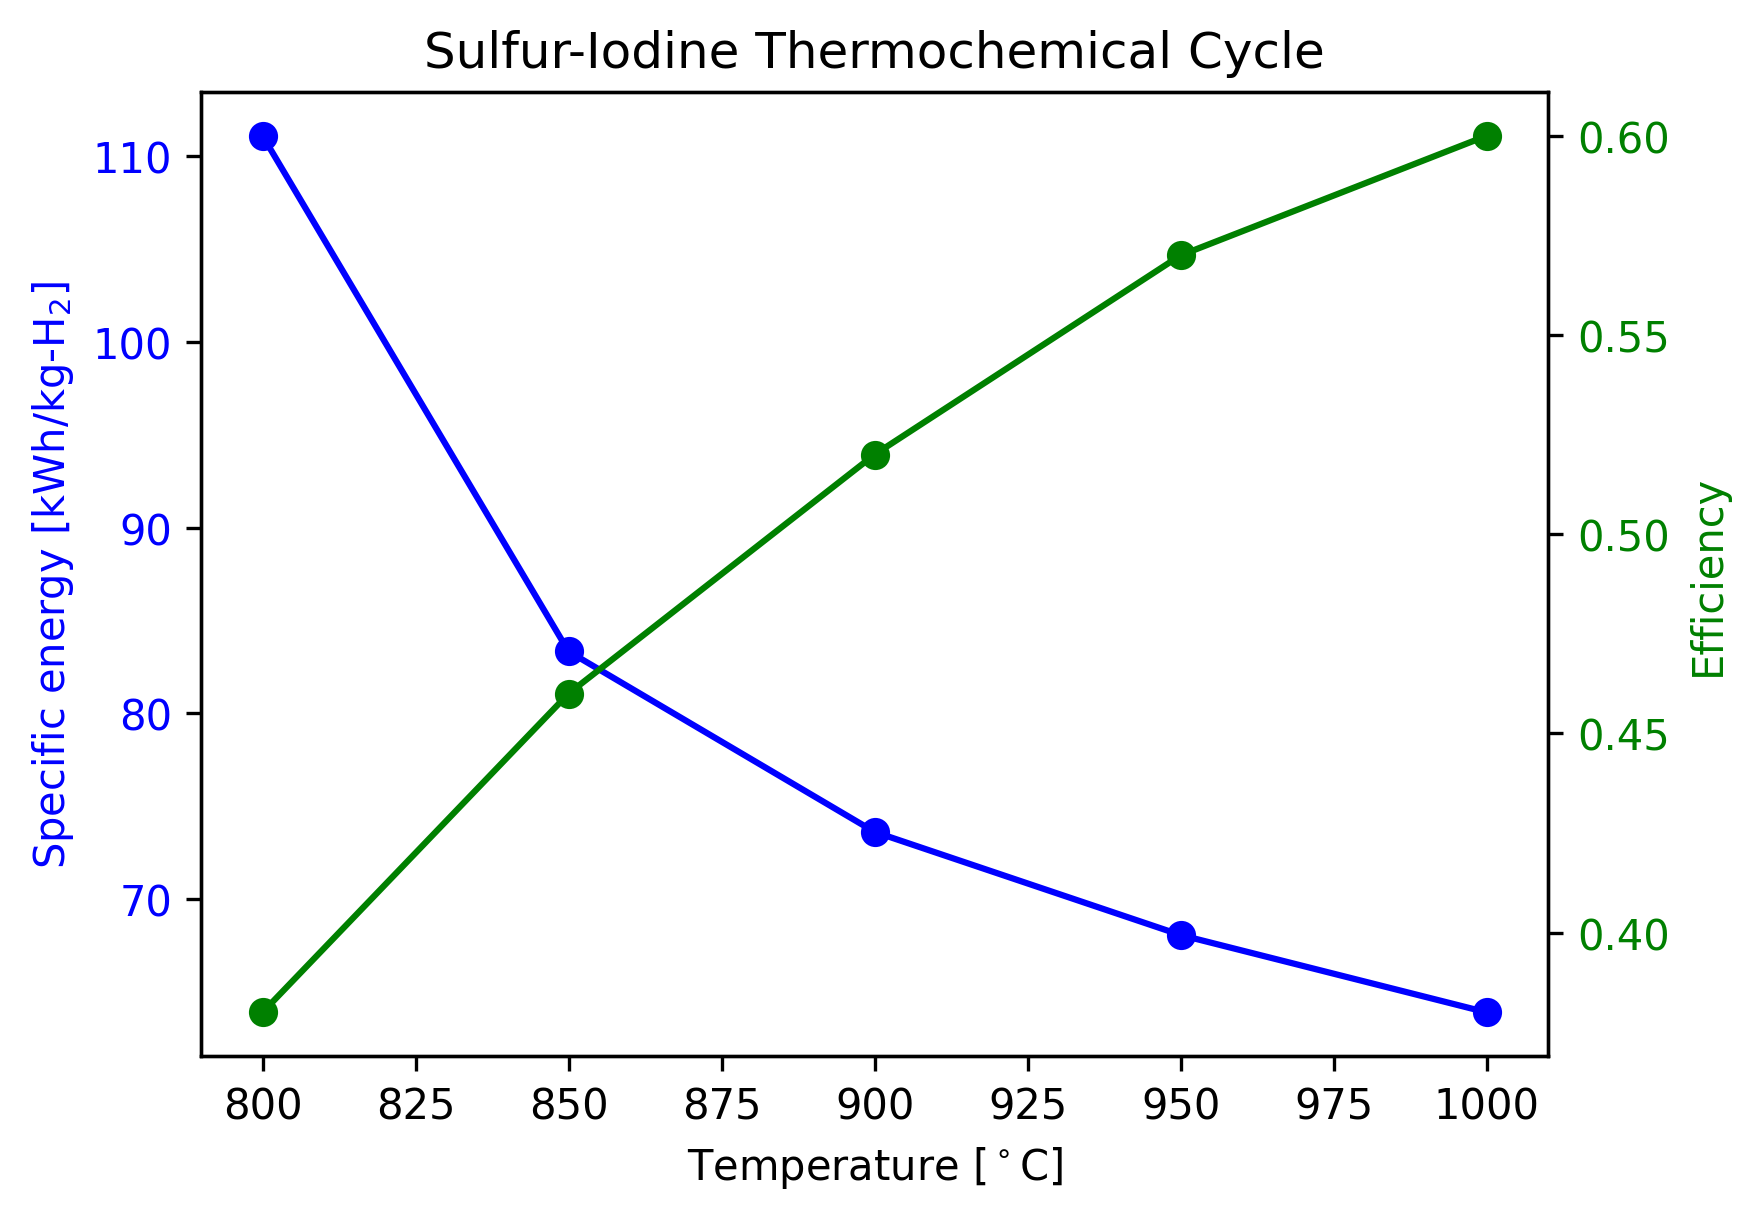
\includegraphics[width=4.8cm]{images/si-energy2.png}
		\end{center}
		\caption{Energy required by the Sulfur-Iodine Thermochemical Cycle.}
 	\end{figure}
\end{columns}
\end{frame}

\begin{frame}
\frametitle{Co-generation}
\begin{columns}
    \column[t]{5cm}
  	\begin{figure}[htbp!]
		\begin{center}
			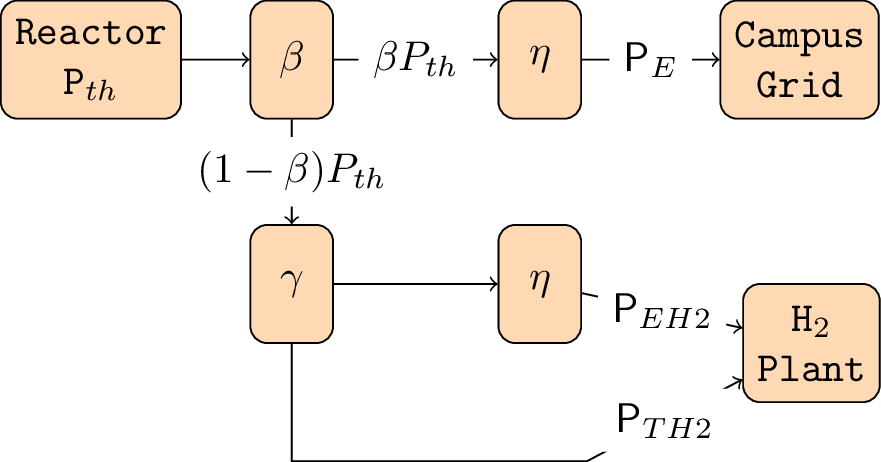
\includegraphics[width=4.5cm]{images/hte-figure0.png}
		\end{center}
		\caption{Diagram of a reactor coupled to a hydrogen plant.}
 	\end{figure}

 	\column[t]{5cm}
	\begin{table}[!htb]
		\centering
	    \caption{Energy requirements of the different H$_2$ production methods.}
		\begin{tabular}{cccc}
	\hline
    Method    & $\gamma$         & $P_{EH2}$ & $P_{TH2}$ \\ \hline
    LTE & 1                & $\ne$ 0   & 0         \\ 
    HTE & $0 < \gamma < 1$ & $\ne$ 0   & $\ne$ 0   \\ 
    SI  & 0                & 0         & $\ne$ 0   \\ \hline
        \end{tabular}
	\end{table}
\end{columns}
\end{frame}

	% \begin{table}[!htb]
	% 	\centering
	%     \caption{GGE, DGE, and E85GE \cite{doe_office_of_energy_efficiency_and_renewable_energy_hydrogen_2020} \cite{alternative_fuels_data_center_fuel_2014}.}
	% 	\begin{tabular}{l|l}
	% 	\hline
	% 	                 & Hydrogen \\ \hline
	% 	GGE              & 1 kg     \\
	% 	DGE              & 1.13 kg  \\
	% 	E85GE            & 0.78 kg  \\ \hline
 %        \end{tabular}
	% \end{table}